\chapter{Background}\label{BackgroundLit}
This chapter will review the necessary concepts of quantum computing that are required in order to further explore the modular approach. 
A circuit consists of data, operations and results, these components provide the context for the following segment.


\section{Qubit} \label{QubitBackG}

Similar to bits found in classical computers, a quantum bit or qubit is the smallest unit of measurement in a quantum computer. Using the Dirac Vector notation or the Bra-Ket notation \citep{wikiVec}, we can represent a qubit in state zero as $|0\rangle$ with $|1\rangle$ for a qubit in state one. These can be denoted in vector form as:



\begin{equation}
    \begin{tabular}{p{3cm}p{3cm}}
        $|1\rangle$ = 
            $\begin{bmatrix}
                0 \\
                1
            \end{bmatrix}$
        & 
        $|0\rangle$ = 
           $\begin{bmatrix}
                1 \\
                0
            \end{bmatrix}$
    \end{tabular}
\label{qubitVector}
\end{equation}



Two qubits can be represented in a four-dimensional linear vector space that holds the probability amplitudes of each possible state. These are spanned by the following product basis states: 

%%%%%%%%%%%%%%%%%%%%%%%%%%%%%%%%%%%%%%%%
\begin{figure}[H]
      \centering
      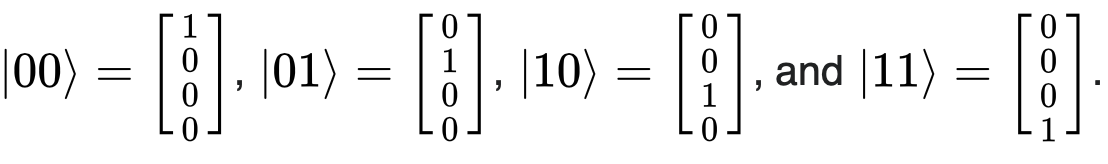
\includegraphics[scale=0.6]{background/fourVec.png}
      \caption{Two Qubit Vector Representation \citep{wikiVec}}
      \label{fourVec}
\end{figure}
%%%%%%%%%%%%%%%%%%%%%%%%%%%%%%%%%%%%%%%%

\subsubsection*{Bloch Sphere}

The geometrical representation of a qubit is usually illustrated using the Bloch sphere. The Bloch sphere is a two level system consisting of a northern and southern hemisphere. 
The north pole of the sphere is assigned the state $\vert0\rangle $ and the south pole the state $\vert 1\rangle $. A classical bit would be represented on the Bloch sphere as being in either the north pole of the sphere or the south pole. A qubit however, can be a point anywhere on the surface of the sphere \citep{he2003}.

%%%%%%%%%%%%%%%%%%%%%%%%%%%%%%%%%%%%%%%%
\begin{figure}
      \centering
      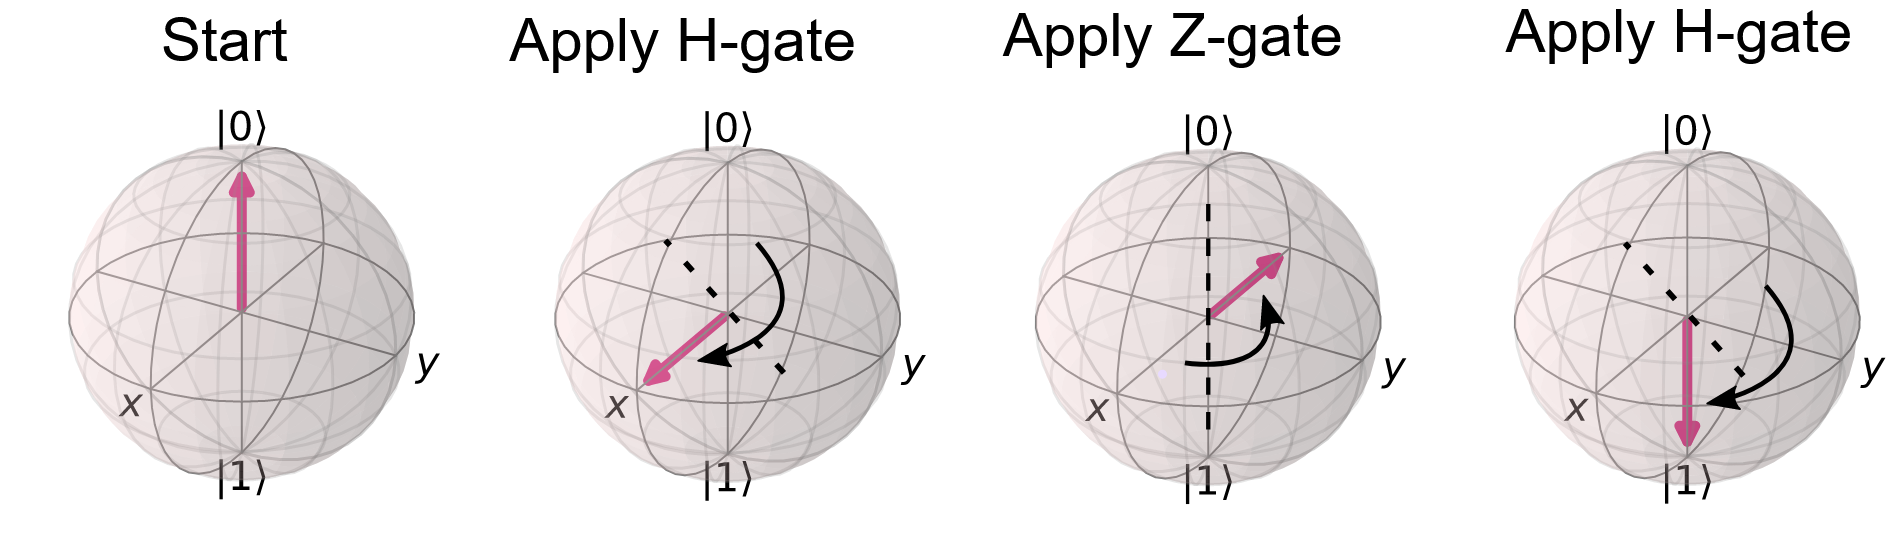
\includegraphics[scale=0.5]{background/blochS.PNG}
      \caption{Transcription within Bloch Sphere with respect to gate operation \cite{theJBC}}
      \label{fourBlokVec}
\end{figure}
%%%%%%%%%%%%%%%%%%%%%%%%%%%%%%%%%%%%%%%%

When encoding classical data into a quantum space, a data point is represented as an angle. Referring to Figure \ref{fourBlokVec}, the angle is then mapped to a coordinate within the Bloch sphere. 
 However, the Bloch sphere is not a precise indicator of where a qubit lies on the unit sphere, it merely shows the latitude of the qubit. The latitude defines how close the qubit is to the poles, depending on the probability amplitudes \citep{he2003}.

\subsection{Entanglement and Superposition}

\subsubsection*{Superposition}

Classical bits always have a completely well-defined state: they are either 0 or 1 at every point of a computation. The difference between a qubit and a classical bit is the possibility for a qubit to be in a linear combination of states, denoted by;

\begin{displaymath}
\vert\phi\rangle = \alpha\vert0\rangle + \beta\vert 1\rangle  
%\cite{he2003}%
\label{eq:s}
\end{displaymath}


The values $\alpha$ and $\beta$\ are complex numbers and their ability to exist in multiple states is called superposition.



\subsubsection*{Entanglement}

Quantum machines do not allow the amplitudes of $\alpha$ and $\beta$\ to be directly viewed. A qubit can therefore encode an infinite amount of information, but most of this information is useless as it can never be observed \citep{he2003}. 
In order to observe the state that a qubit is in, a measurement is performed. 


Taking a two qubit system, there are four basis states that they can collapse to, which are  $\vert00\rangle $,  $\vert01\rangle $, $\vert 10\rangle $ and $\vert 11\rangle $.
These states are referred to as the Bell States or EPR states \citep{he2003}. An example of one of these states is the following (from \cite{he2003}):

\begin{displaymath}
\vert\phi\rangle = \frac{\vert00\rangle + \vert 11\rangle }{\sqrt(2)}
\end{displaymath}

When the first qubit is measured, there are two possible results: 

If the first qubit is in state 0, it provides the probability of the other qubit residing in state $\vert00\rangle $ as 1/2.

If the first qubit is in state 1, it  also produces the probability of the other qubit residing in state $\vert 11\rangle $ as 1/2. 

This means that when the second qubit is measured it will always be in the same state as the first qubit. This correlation between the qubits is known as entanglement \citep{he2003}. 

\subsection{Quantum Gates}

Quantum logic gates or simply quantum gates are the building blocks of a quantum circuit. They can be used to manipulate and transform qubit states. 
Quantum gates are briefly described here, for a more in depth treatment of this topic please refer to \emph{Quantum computing for computer scientists} \citep{yanofsky2008quantum}.

\textbf{Hadamard gate or the H gate:} The Hadamard gate is defined by the unitary matrix:

%%%%%%%%%%%%%%%%%%%%%%%%%%%%%%%%%%%%%%%%
\begin{figure}[h!]
      \centering
      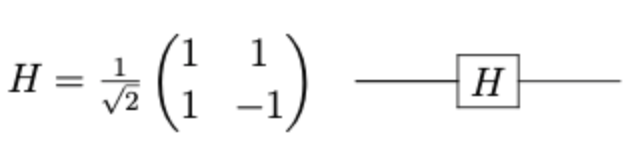
\includegraphics[scale=0.7]{background/HGate.png}
      \caption{Hadamard Gate
      \citep{Khan2019}}
      \label{HGa}
\end{figure}
%%%%%%%%%%%%%%%%%%%%%%%%%%%%%%%%%%%%%%%%


It is objectively one of the most important gates, as it serves to place qubits in equal superposition of  $\vert0\rangle $and  $\vert1\rangle $.
%%When applied to one qubit it maps maps the basis state%% 


\vspace{0.5cm}
\textbf{NOT gate or the X gate:} The NOT gate is the quantum equivalent of the NOT gate found in classical computers. It  flips the probabilities of state $\vert0\rangle $ and  $\vert1\rangle $.

%%%%%%%%%%%%%%%%%%%%%%%%%%%%%%%%%%%%%%%%
\begin{figure}[H]
      \centering
      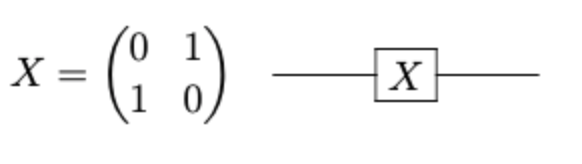
\includegraphics[scale=0.7]{background/NotGate.png}
      \caption{NOT Gate
      \citep{Khan2019}}
      \label{NotGa}
\end{figure}
%%%%%%%%%%%%%%%%%%%%%%%%%%%%%%%%%%%%%%%%

\textbf{Identity gate or the ID gate:} The Identity gate is a single-qubit operation that leaves the basis states $\vert0\rangle $ and  $\vert1\rangle $ unchanged. It ensures that no operation occurs on the qubit for one unit of time.
\begin{equation*}
\centering
I = 
\begin{bmatrix}
1 & 0 \\
0 & 1
\end{bmatrix}
\end{equation*}

\textbf{Controlled NOT or CNOT gate:} The CNOT gate acts on two qubits and performs the NOT operation on the second qubit only when the first qubit is $\vert1\rangle $, otherwise it leaves it unchanged \citep{wikiVec}. 

%%%%%%%%%%%%%%%%%%%%%%%%%%%%%%%%%%%%%%%%
\begin{figure}[h!]
      \centering
      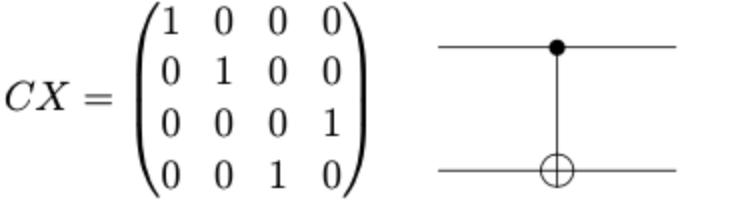
\includegraphics[scale=0.6]{background/CNOTGate.png}
      \caption{Controlled NOT Gate
      \citep{Khan2019}}
      \label{CNotGa}
\end{figure}
%%%%%%%%%%%%%%%%%%%%%%%%%%%%%%%%%%%%%%%%

\vspace{0.5cm}

\textbf{Toffoli (Controlled Controlled Not gate [CCNOT]):} The Toffoli gate is a three-qubit gate in which two qubits act as a control and the third qubit is the target. If both of the control qubits are in state $\vert1\rangle $ then the target qubit is flipped and the control qubits remain unchanged \citep{Khan2019}.

%%%%%%%%%%%%%%%%%%%%%%%%%%%%%%%%%%%%%%%%
\begin{figure}[h!]
      \centering
      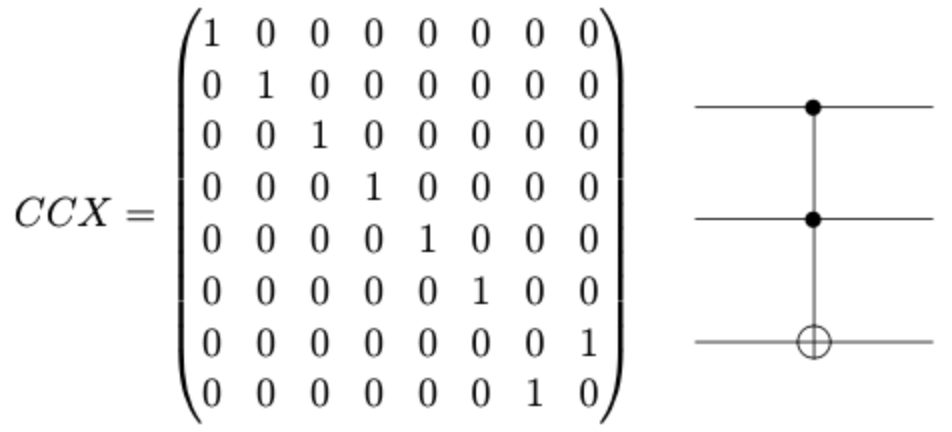
\includegraphics[scale=0.6]{background/TGate.png}
      \caption{Toffoli Gate
      \citep{Khan2019}}
      \label{ToGa}
\end{figure}
%%%%%%%%%%%%%%%%%%%%%%%%%%%%%%%%%%%%%%%%

\textbf{Rotation Y or Ry gate:}
The Ry gate rotates the qubit along the y-axis to the specified angle $\Theta$ within the Bloch sphere. This can be useful for mapping classical data points into a quantum space\vspace{0.8cm}.


%%%%%%%%%%%%%%%%%%%%%%%%%%%%%%%%%%%%%%%%
\begin{figure}[h!]
      \centering
      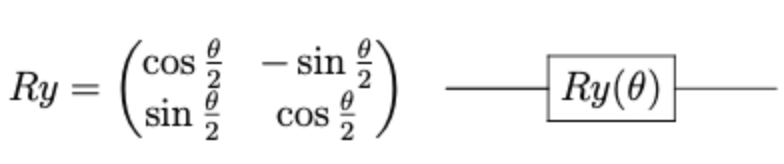
\includegraphics[scale=0.7]{background/RGate.png}
      \caption{Rotation Y Gate
      \citep{Khan2019}}
      \label{RYGa}
\end{figure}
%%%%%%%%%%%%%%%%%%%%%%%%%%%%%%%%%%%%%%%%


\textbf{SWAP  gate:} The SWAP gate is a two-qubit operation that swaps the state of the qubits involved in the operation.
%%%%%%%%%%%%%%%%%%%%%%%%%%%%%%%%%%%%%%%%
\begin{figure}[h!]
      \centering
      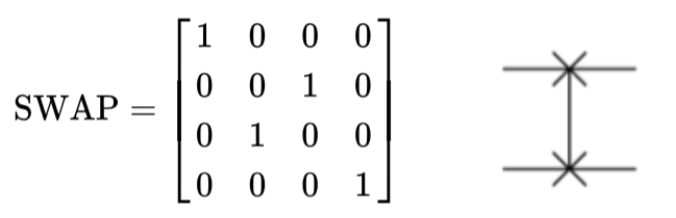
\includegraphics[scale=0.6]{background/SWAPG.png}
      \caption{SWAP Gate}
      \label{SWAPLogic}
\end{figure}
%%%%%%%%%%%%%%%%%%%%%%%%%%%%%%%%%%%%%%%%


As shown in Figure \ref{SWAPGa}, the SWAP gate allows us to move information around in a quantum circuit without effecting the qubit data. %explain diagram 

%%%%%%%%%%%%%%%%%%%%%%%%%%%%%%%%%%%%%%%%
\begin{figure}[H]

       \centering
      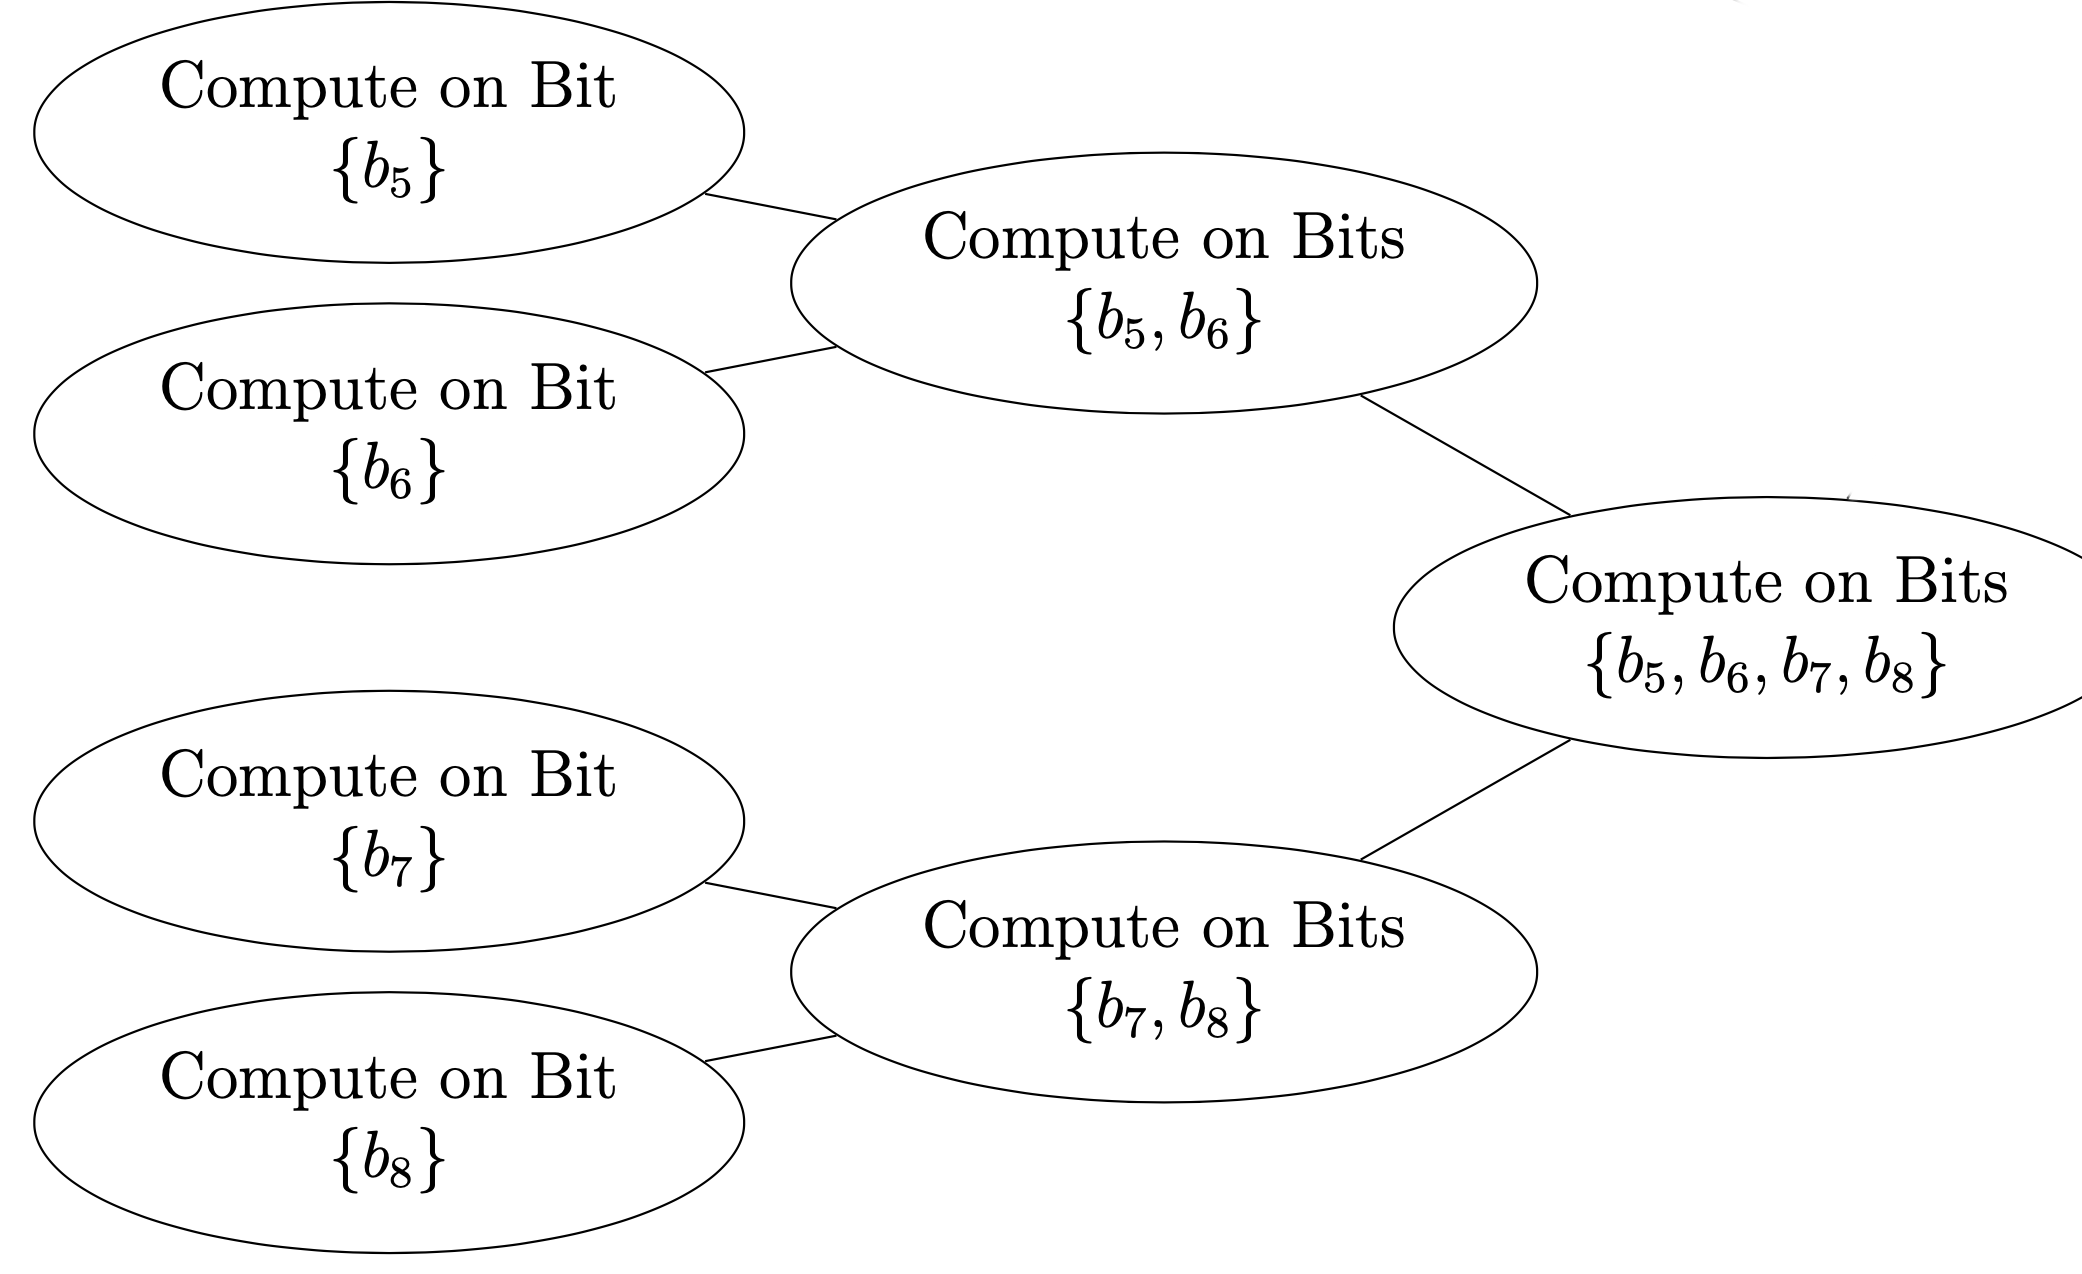
\includegraphics[scale=0.2]{background/SWAP.png}
      \caption{SWAP Gate Process
      \citep{Cortese}}
      \label{SWAPGa}
\end{figure}
%%%%%%%%%%%%%%%%%%%%%%%%%%%%%%%%%%%%%%%%



\section{Quantum Data Encoding}
With the knowledge of how bits are represented, an understanding of how classical data is stored on quantum bits is needed as encoding data in qubits is not trivial. Current quantum devices contain a limited amount of qubits that are stable for a short amount of time \citep{DataEn}. In order to make use of current quantum devices our circuit representation must be compact and limited to a set amount of qubits and quantum gates. To do so we will exercise quantum data encoding or data embedding. These techniques allow us to take a classical data point, $x$, and encode it by applying a set of gate parameters on the quantum circuit. The operations that will be performed depend on the value of $x$, hence creating the desired quantum state.

There exist different methods for data encoding, an example of these are:

\textbf{Basis Encoding:} This is categorised as a digital encoding technique because it is suitable for arithmetic computations \citep{Leymann}. In this method, data is simply encoded into binary strings, where each input is converted to a computational basis state of a qubit system. 
While this provides a lot of freedom computationally, the available implementation schemes are usually not efficient \citep{rodneyD}.



\textbf{Angle Encoding:} In this type of encoding, classical information is encoded into angle rotations of a qubit. This results in using the feature values of an input data point, $x$, as angles in a unitary quantum gate \citep{rodneyD}.

This discourse makes use of amplitude encoding and feature mapping to encode classical data. 

\subsection{Amplitude Encoding}\label{AmpEnBack}

Amplitude Encoding can also be referred to as Wavefunction Encoding \citep{LaRoseC}. It consists of mapping the coordinates of a vector into the values of the amplitudes of a quantum state. It requires the vector to be normalised and to have a power-of-two dimensions \citep{slimaneT}. 

Section \ref{PrepData} implements an example of when these conditions are not fulfilled by the dataset, resulting in the need to pad and re-normalise the vector. This is carried out by preparing the data through normalisation and feature padding; the datapoint angles are then extracted from this prepared data. The extracted angles are then rotated to encode them within the Bloch sphere and this encoding allows the data to be encoded into a quantum state. 

This type of data encoding is very useful for smaller datasets with multiple features, as it does not map each feature to a specific qubit. However, it does take multiple steps to encode the data, and with larger datasets this could increase resource requirements.  

%This method is also intuitive however, schemes to implement it can be complicated. When observing the current literature it difficult to implement amplitude encoding solely from the illustrations

\subsection{Feature Mapping}\label{FMapBack}
A feature map reduces the amount of resources required to describe a large set of data as it maps this data into a higher dimensional space or quantum Hilbert space \citep{rodneyD}.

\textbf{Hilbert Space:} The Hilbert space is a large space where the states that describe quantum systems live. For a 50-qubit quantum computer, it would be a 1,125,899,907,000,000 - dimensional space. For a single mode of a continuous-variable quantum computer, the Hilbert space has an infinite number of dimensions \citep{mariaS}.

Feature maps encode the classical data by applying the parameterised circuit V($\phi(\overrightarrow{x_i})$, which converts the classical data into quantum data. Where:
 
 $\overrightarrow{x_i}$: Represents the classical data set. 
 
 $\phi$(): Is the classical function applied on the classical data set. 
 
 V: Is the vector space. 
 
 As discussed earlier in Section \ref{QubitBackG}, qubits can be denoted in vector form. Feature maps use this vector notation to encode the classical data $x_i$ into quantum states. 
 
  Section \ref{FMapp} of this dissertation implements three different types of pre-coded feature maps found in the Qiskit circuit library, namely: ZZFeaturemap, ZFeaturemap and PauliFeaturemap. It is possible to vary the depths of these feature maps (1, 2, 4) in order to check a models performance. By increasing a feature map’s depth, we introduce more entanglement into the model \citep{rodneyD}. 

\section{Quantum Circuit Application}
This section builds on the knowledge of circuit components and data encoding by utilising them to express operations. It first needs to be established, which quantum operations or circuits one wishes to implement. 
%However, an understanding into type of quantum operations/ circuit that will be needed must be established.

\subsection{Quantum k-Nearest Neighbour (QkNN)}\label{QkNNexplain}

The k-Nearest Neighbour algorithm is a simple supervised machine learning algorithm that is used extensively for pattern recognition and classification \citep{kNNToward}. When  given a testing sample, the algorithm find its k nearest neighbours based on some distance metric and then determines its category according to the information of these neighbours. 

There exists different quantum k-Nearest Neighbour implementations, one such example, that is explored later in this work, is the Hamming Distance. %which is be explored later in this work. %which will later in this work we will explore the Hadamard Distance implementation.

\vspace{0.4cm}
\textbf{\underline{Quantum k-Nearest Neighbour Algorithm Using Fidelity}}

 QkNN using \emph{fidelity} \citep{QKNAll} performs a SWAP test between the test states and all training states in superposition to analog-encode the fidelity. The SWAP test is a quantum algorithm that can be used to statistically estimate the fidelity of the two pure states $\vert\psi\rangle$ and $\vert\phi\rangle$ as follows:

\begin{enumerate}
\item 
An initial preparation of three registers in states $\vert0\rangle$, $\vert\psi\rangle$,  $\vert\phi\rangle$ is needed in order to implement the SWAP test. This results in an initial combined state of the three registers as:  $\vert R\rangle$ = $\vert0\rangle$ $\otimes$ $\vert\psi\rangle$ $\otimes$ $\vert\phi\rangle$ \citep{QML}.
\item
Then a initial Hadamard operation is applied on the first register followed by a control SWAP on the other two registers, with the first register serving as the control in the system \cite{QML}.
\item
 Lastly, another Hadamard operation (H) is applied on the first qubit {$\vert0\rangle$, $\vert1\rangle$}, resulting in 0 and 1 with the probabilities: 
\end{enumerate}
%%%%%%%%%%%%%%%%%%%%%%%%%%%%%%%%%%%%%%%%
\begin{figure}[h!]
      \centering
      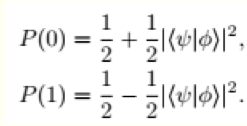
\includegraphics[scale=0.44]{background/KNFid.png}
      \caption{Quantum K-Nearest Neighbour Using Fidelity
      \citep{QML}}
\end{figure}
%%%%%%%%%%%%%%%%%%%%%%%%%%%%%%%%%%%%%%%%

The quantity $P(0) - P(1)$ gives us the desired fidelity \citep{QML}.

\vspace{0.4cm}
\textbf{\underline{Quantum k-Nearest Neighbour Algorithm Using Hamming Distance }}

Section \ref{ImpleQkNN} implements the Hamming distance QkNN as described in \emph{Quantum Algorithm for K-Nearest Neighbours Classification Based on the Metric of Hamming Distance} \citep{HammInstruct}.

After the necessary data encoding steps, the condition of the Hamming distance is sought. The Hamming distance is defined as counting the differing number of corresponding symbols in two bit-vectors of equal length e.g:
 
 Hamming Distance: 0110 $\leftrightarrow$ 0001, has a distance of 3.
 
 Hamming Distance: 0110 $\leftrightarrow$ 1110,  has a distance of 1.
 
The condition of the Hamming distance is retrieved by applying two quantum additions and a quantum OR operation to the most significant bit. This results in a zero or one output, which indicates the presence of a neighbour. 

When using the classical kNN algorithm on larger data sets, there is a noticeable degradation in the performance of the algorithm. 
Quantum k-Nearest Neighbour places the entire the training set into superposition at the very start. Thus, in one run it can calculate all distances between the input and the entire training set. This allows the circuits to only require as much qubits as is needed to encode the entire training set.


\subsection{ Quantum Support Vector Mechanism (QSVM)}

Support Vector Mechanism(SVM) is a form of supervised learning used to classify data into categories. SVM takes a training dataset and virtually plots the data in d-dimensional space, where d is the number of parameters or features of each data point. It then attempts to find the (d-1)-dimensional hyper-plane which separates the data into two classes \citep{C18}. %In a case of data with two parameters this is a line.

In many cases it is impossible to draw a separating hyperplane between classes of data, especially when the boundary is highly nonlinear \citep{C18}. In such a case where the SVM is unable to find a suitable separating hyperplane, a technique known as a kernel trick is used \citep{qmlCovid}. The kernel rick uses a nonlinear function or a feature map to project the data into a higher dimension where a separating hyperplane may be found \citep{C20}.

In the case of  the Quantum Support Vector Mechanism(QSVM) used by \emph{\citep{mcrae2020}}, only the quantum feature maps V($\phi(\overrightarrow{x_i})$) is used to translate the classical data $\overrightarrow{x}$ into quantum states. The kernel for the SVM is built out of these quantum states. After calculating the kernel matrix using quantum mapped data, the quantum SVM can then be trained in the same fashion as the classical SVM \citep{svm}.


The idea of the quantum kernel is exactly the same as the classical case where the inner product of the feature map K($\overrightarrow{x}, \overrightarrow{z}$)= $\vert\langle\Phi(\overrightarrow{x})\vert\Phi(\overrightarrow{z})\rangle\vert^2$, is taken but with the quantum feature mapped data in replacement.%$The idea of choosing a quantum feature map that is not easy to simulate with a classical computer, could obtain a quantum advantage \citep{svm}.

%With this logic we can build out a quantum circuit following the work of from [cite].%

Section \ref{QSVMImp} will reveal how to make use of the predefined functions provided by Qiskit Aqua to implement QSVM. These functions will require the feature map, a training and a test set as inputs, in order to train the whole QSVM.

\vspace{0.4cm}
\textbf{\underline{QSVM Quantum Advantage }}

The quantum version of the SVM is best described as “quantum-assisted” or “quantum-enhanced” \citep{Back7}, in the sense that the algorithm is largely classical with certain operations performed by a quantum processor.

In the case of a quantum SVM, the quantum feature maps are used to translate the classical data into quantum states. The classical kernel used for SVM is then built out of these quantum states, which are then used to train the QSVM in the same way as the classical SVM.

QSVM will minimise the loss via optimising the parameters. However, apart from finding the quantum kernel data, the QSVM algorithm preforms only classical optimisation. In the end there is no significant difference between the QSVM and the classical SVM.


\subsection{Grover's Search Algorithm }\label{GrovImp}
This section will introduce Grover's Search algorithm and how it can be used to solve unstructured search problems.


Grover's Search algorithm is named after the creator Lov Kumar Grover. It is a quantum computing algorithm that can search databases much faster than a classical computer. Grover's Search algorithm can speed up an unstructured search problem quadratically. It is one of the first and most prominent examples to showcase how a quantum circuit can be magnitudes faster than a classical algorithm \citep{FrankZ}. As it takes $O(N1/2)$ time, while a linear search, which is $O(N)$ time. As such, it is the fastest possible quantum algorithm for searching an unsorted database. 

Although the purpose of Grover's Search algorithm is usually described as searching a database, it may be more accurate to describe it as inverting a function. Taking a function $y=f(x)$, that can be evaluated on a quantum computer, Grover's Search algorithm allows for the calculation of $x$ when given $y$. Inverting a function is related to the searching of a database as it can create a function that produces a particular value of $y$ if $x$ matches a desired entry in a database, and another value of $y$ for other values of $x$ \citep{GroversEx}. \citeauthor{EvaB}\emph{ Grover Search algorithm} \citep{EvaB}, provides a more in-dept exploration into the inner workings of Grover's Search algorithm.

Grover's Search algorithm can also be used for estimating the mean and median of a set of numbers, and for solving the collision problem. In addition, it can be used to solve NP-complete problems by performing exhaustive searches over the set of possible solutions. 

The application of Grover's Search results in "only" a quadratic speedup, unlike other quantum algorithms, which can provide exponential speedup over their classical counterparts. However, this quadratic speed-up becomes considerable when $N$ is large.


%This quadratic speed up would result in a considerable speedup over classical solutions \citep{GroversEx}. 



\section{Quantum Computers}
The final step in quantum circuit as illustrated in Figure \ref{ImpleLayout} is the measurement step. If we think of Schrödinger’s cat, which can be dead or alive with some probability, opening the box is “measuring” the state of the cat. In the same way, quantum computers estimate the probability of a qubit belonging to a class by performing certain measurements. 

%This is the equivalent of sampling multiple times from the distribution of possible computational basis states and obtaining an expectation value. 
To carry out this measurement would require executing our circuit on a quantum computer. However, quantum computers are expensive and costly to maintain, as such we will make use of cloud-based quantum computers. 


Cloud-based quantum computing allows companies, researchers and individuals to test their quantum algorithms. Cloud-based quantum computing achieves this by providing direct access to emulators, simulators and quantum processors. Vendors also provide development platforms and documentation for quantum computing languages and tools \citep{QCloudC}.

\subsection{Quantum Machines}

Cloud-based quantum machines provide an environment for businesses and academia to practice quantum approaches without having to wait for quantum computing technology to mature and become more widespread \citep{QCloudC}.

%There exist many quantum cloud computing vendors and 
Here are some of the more prominent cloud-based quantum computing providers:

\textbf{D-Wave Systems:} Founded in 1999, D-Wave is one of the earliest players in quantum computing. They were the first company to provide a commercially available quantum computer. However, the D-Wave machine has very weak coherence times, and the range of Hamiltonians\footnote{The Hamiltonian of a system is an operator corresponding to the total energy of that system, including both kinetic energy and potential energy. \citep{wikiHamilton}} %A Hamiltonian is a function that is used to describe a dynamic system (such as the motion of a particle) in terms of components of momentum and coordinates of space and time and that is equal to the total energy of the system when time is not explicitly part of the function}
 they can produce is limited. This results in the D-Wave device(s) being more suited to use as a quantum enhanced annealer \citep{QCloudC}.

Quantum annealing is a quantum computing method used to find the optimal solution of problems involving a large number of solutions, by taking advantage of properties specific to quantum physics like quantum tunneling, entanglement and superposition \citep{QAnnealing}. It is often used, in preference to other methods, to find the global minimum of a given object function.

In the current research landscape, quantum annealing is used for optimisation machine learning problems in four broad areas \citep{nath2021review}:
\begin{enumerate}[(i)]
\item Image Recognition
\item Remote Sensing Imagery 
\item Particle Physics 
\item Computational Biology. 
\end{enumerate}
%as
%\emph{``Quantum annealing could be a better choice for training ML classifiers in the presence of limited training data''.} 
It is noted that \emph{``Machine learning tasks using quantum annealing are performed in a hybrid classical and quantum system''}. The use of D-Wave's quantum annealing system would allow for the implementation of a hybrid QSVM algorithm but the implementation of a full quantum QkNN algorithm may not be currently feasible \citep{nath2021review}. %with a quantum annealer.

\textbf{Google’s Quantum Playground:} Google's Quantum Playground provides a simulator with a user interface, scripting language and 3D quantum state visualisations. Along with this, Google announced the achievement of quantum supremacy by using a 54-qubit Sycamore processor in late 2019 \citep{QCloudC}.  %in Playground. 
Although the platform offers access to TensorFlow Quantum, which is a library for building quantum machine-learning models, they have not yet included a general-purpose quantum computing service.


\textbf{Microsoft Quantum Computing:}  Microsoft provides 
%tools such as 
Quantum Development Kits (QDK) and a quantum script language called $Q\#$ for quantum computing development.  $Q\#$ is a C$-$style programming language consisting of a \emph{``set of libraries that abstract complex functionality in $Q\#$, APIs for Python and .NET languages ($C\#$, $F\#$, and VB.NET) for running quantum programs written in $Q\#$, and tools to facilitate your development''} \citep{LaRos2019}. Microsoft partnered with 1Qbit, Honeywell, IONQ and QCI during the development of their quantum computing systems. Microsoft has also developed their own quantum system called Station Q \citep{QCloudC}.

The Microsoft QDK was not used for this dissertation implementation because it lacks support for a SWAP gate to move quantum information around a quantum circuit \citep{LaRos2019}.
Additionally it could be argued that Python is a more approachable language than a C$-$style language such as $Q\#$ . %and QDK lacks support for a SWAP gate to move quantum information around a quantum circuit \citep{LaRos2019}, Microsoft QDK was not used for this dissertation implementation. 

\textbf{IBM Q Experience:} IBM introduced a quantum network called IBM Q network in 2016. Since then, IBM became one of the forerunners in the quantum computing ecosystem. IBM Q can be accessed on the cloud through Qiskit, which is an open-source quantum software development kit \citep{QCloudC}.

This work will make use of IBM’s Qiskit network. While Qiskit does not support quantum annealing like the D-Wave system and it has not reached quantum supremacy like Google, Qiskit has many other advantages. These include having a large and active open source community, its documentation is slightly more centralised and Qiskit supports third party simulators, which are all necessary components for this modular tool.


\subsection{Errors, Noise and Interference} \label{NoiseErrInter}
Unlike classical computers which are known for their predictable determinism, quantum computers are inherently probabilistic by nature \citep{ERNIStar}. This section will explore how quantum computers are made even less predictable through quantum errors, noise, interference and decoherence. 

\vspace{0.4cm}
\textbf{\underline{Quantum Errors}}\label{ERNoi}

Errors can be caused by noise and environmental interference. However, they are generally caused by the flawed execution of operations, such as quantum logic gates and measurement operations, as well as decoherence \citep{ERNIStar}.
There also exists spectator errors or crosstalk, this is when an operation on one qubit can have an unintended effect on a nearby qubit. Using ID gates on qubits that one does not intended to have operations running on, can slightly reduce this possibility. However, this will only aim to reduce these types of errors and not mitigate them from existing within the quantum process.

%\vspace{0.4cm}
%\textbf{\underline{Quantum Interference and Decoherence}}

%Quantum machines can only predict the probability of a certain outcome, with the final probability being assumed during the measurement stage.
%Quantum interference is a byproduct of superposition, in that it can be used to reinforce the probability of obtaining the desired result, all while reducing unwanted results via constructive or destructive interference \citep{INGKOK}. A disruption in quantum interference can be a source of error, this type of disruption is called decoherence.


%\textbf{Decoherence:} Decoherence refers to the fact that gradually over time a quantum computer has the probability to behave more like a classical object. After decoherence has fully occurred, the computer can no longer take advantage of quantum effects, this introduces progressively more noise as the quantum algorithm proceeds \citep{ColesQuantumAIC20}.

\vspace{0.4cm}
\textbf{\underline{Quantum Noise}}

When implementing a quantum algorithm it is important to consider the sources of the noise. % in the computer. 

Noise differs from environmental noise in that the source of the noise comes from within the quantum machine itself. These include electrical and mechanical components, cabling, wiring, circuit connections, and intermittent interactions of any of the preceding \citep{ERNIStar}. Environmental noise can stem from \emph{``uncontrolled interactions between system and environment, such as thermal motion of charge carriers or stray magnetic fields, lead to deviations between the targeted and the actual evolution''} \citep{QEnviron}; which in turn can lead to a loss of coherence in the system. 

The two main sources of noise are typically gate infidelity and decoherence. 
%‘Environmental’ decoherence is decoherence that arises through suitable interaction of a system with its environment.

\textbf{Gate Infidelity:} The more qubits present in a system, the higher the probability that one qubit will loose too much information, this can cause the entire circuit to become useless. The number of qubits required to execute a quantum circuit depends on the complexity of the circuit. Therefore, large quantum circuits constructed using many qubits are more susceptible to noise \citep{INGKOK}.

%\textbf{Decoherence:} Decoherence refers to the fact that gradually over time a quantum computer has the probability to behave more like a classical object. After decoherence has fully occurred, the computer can no longer take advantage of quantum effects, this introduces progressively more noise as the quantum algorithm proceeds \citep{ColesQuantumAIC20}.

\vspace{0.4cm}
\textbf{\underline{Quantum Interference and Decoherence}}

Quantum machines can only predict the probability of a certain outcome, with the final probability being assumed during the measurement stage.
Quantum interference is a byproduct of superposition, in that it can be used to reinforce the probability of obtaining the desired result, all while reducing unwanted results via constructive or destructive interference \citep{INGKOK}. A disruption in quantum interference can be a source of error and this type of disruption is called decoherence.


\textbf{Decoherence:} Decoherence refers to the fact that gradually over time a quantum computer has the probability to behave more like a classical object. After decoherence has fully occurred, the computer can no longer take advantage of quantum effects and this introduces progressively more noise as the quantum algorithm proceeds \citep{ColesQuantumAIC20}.

\vspace{0.4cm}
\textbf{\underline{Error, Noise and Interference Correction}}

There are methods available that can reduce error, noise and interference.

\textbf{Shots:} When executing our quantum circuit we can specify the number of shots. These shots are effectively the number of repetitions the circuit will undertake with the intention that environmental interference and possibly noise and errors will be removed to some degree. 

\textbf{Quantum Error Correction:}\label{QEC} Quantum Error Correction (QEC) is used to protect quantum information from errors that are primarily due to decoherence and quantum noise. Quantum error correction is essential in order to achieve fault-tolerant quantum computation that can deal not only with noise found in stored quantum information but also with faulty quantum gates, faulty quantum preparation and faulty measurements \citep{wikiERI}.

While QEC is in the early stages of development, it acts by protecting the information stored in qubits by not storing this information in individual qubits but rather in patterns of entanglement among many qubits. More information can be gathered about quantum error correction in \emph{Simon J. Devitt, William J. Munro, and Kae Nemoto work, Quantum Error Correction for Beginners} \citep{Devitt_2013}.

\subsection{Quantum Simulators}
Quantum simulators enable us to simulate both quantum inherent algorithms such as Grover's Search and the quantum counterpart of classical machine learning algorithms e.g QkNN, without loosing the benefits that a quantum environment supplies and in an ideal quantum space without noise.

\vspace{0.4cm}
\textbf{\underline{The JKU Simulator:}}
Qiskit is designed to include third-party simulators that are usually contributed by the quantum open source community. A prime example of such a simulator is the JKU simulator created by Alwin Zulehner and Robert Wille from the quantum computation team at Johannes Kepler University in Linz,
Austria \citep{navehC21}.


This simulator stores quantum states using a data structure which is based on classical decision diagrams. This representation is more complex than simply storing a state vector, rather the vector has regular multiplicities, which then results in a much more efficient storage
space and manipulation time \citep {navehC21}. %All while being able to handle any quantum circuit and not being limited to e.g., Clifford gates\cite {navehC21}.




